\documentclass{article}
\usepackage[utf8]{inputenc}
\usepackage{graphicx}
\usepackage[spanish]{babel}
\usepackage{float}
%%%%%%%%%%%%%%%%%%%%%%%%%%%%%%%
\title{Reporte de la Evaluación 1}
\author{Rolando A. Fimbres G.}
\date{8 de marzo de 2018}
%%%%%%%%%%%%%%%%%%%%%%%%%%%%%%%%%%%
\begin{document}
\maketitle
\section{Descripción}
Se tiene una estación de monitoreo de variables atmosféricas, CO2, radiación solar, nivel de agua y salinidad en el Manglar El Sargento, en una bahía en la costa frente a la parte norte de la Isla Tiburón.\\
Nos interesa explorar los datos de Febrero de 2018 de nivel de mar, salinidad y temperatura del agua. Se proporcionan los datos de cada 15 minutos en formato CSV, que puedes descargar. Nivel de agua: sargento-270218.csv, Salinidad: sargento-salinidad-270218.csv.\\
Se te pide que por favor que crees una carpeta llamada Evaluacion1 en tu espacio de trabajo de Física Computacional 1. Todas las actividades las desarrollarás desde allí.\\
Descarga los archivos de datos de El Sargento a tu carpeta Evaluacion1.\\
Inicia un archivo para el reporte en LaTEX para esta Actividad, donde irás describiendo las actividades realizadas y productos generados.\\
\section{Actividades a Realizar}
1.- Usa los comandos de Linux y Emacs para que los 2 archivos abarquen el mismo periodo de tiempo (mismo rango fechas, mismo número de renglones). Describe brevemente la estructura de los archivos. Cada archivo es generado por un sensor distinto. \\
2.- Ejecuta tu Jupyter Notebook, para leer los dos archivos de datos con el apoyo de Pandas, como lo has hecho con anterioridad. No olvides cargar Pandas, Numpy, Pyplot de Matplotlib y la biblioteca datetime.\\
3.- Con la ayuda de la biblioteca Seaborn,  por favor crea un gráfica de caja (boxplot) para visualizar la variabilidad de los datos de Febrero: a) Nivel de mar (metros); b) Salinidad (Partes por mil - ppt); y c) Temperatura de Agua (ºC).  Con la ayuda de la función describe puedes saber con exactitud la posición de la mediana, cuarteles, máximos y mínimos.\\
4.- De nuevo con la ayuda de Seaborn, también explora si hay una correlación de Pearson entre cada pareja de variables (Regresión lineal con las distribuciones marginales): Nivel de mar-Salinidad, Nivel de mar-Temperatura del agua, Salinidad-Temperatura del agua.\\
5.- Con la ayuda de Matplotlib, realize ahora 3 gráficas independientes de las variables: Nivel del mar, Salinidad y Temperatura del Agua, para ver su variabilidad como función del tiempo.\\
6.- Enseguida, de igual forma, produce gráficas superpuestas con doble eje vertical (izquierda, derecha): a) Nivel de mar y Salinidad; b) Nivel de mar y Temperatura.\\
7.- Con ayuda de la función xlim de pyplot, analiza las gráficas del punto anterior para 5 días y trata de explicar si hay o no una clara manifestación de dependencia de Salinidad y Nivel de mar o de Nivel de Mar y Temperatura del agua.\\
8.- Completa el reporte en LaTEX de la actividad realizada, con segmentos de código y figuras producidas, para después descargar el reporte de actividad en formato PDF a tu carpeta.\\
9.- Como es costumbre sube tu carpeta Evaluacion1 a tu repositorio en Github.\\
%%%%%%%%%%%%%%%%%%%%%%%%%%%%%%%%%%%%%%%%%%%%
\section{Procedimientos Realizados}
Tras crear la carpeta de la evaluación y descargar los archivos en ella, analicé ambos con emacs. Limpié los primeros renglones de ambos para así trabajar solo con números. Después noté que el archivo csv de salinidad comenzaba sus mediciones quince minutos antes y después que el otro archivo. Eliminé ambas filas y continué el análisis en jupyter.\\
Primero cargué los paquetes a utilizar:\\
\begin{figure}[H]
	\centering
    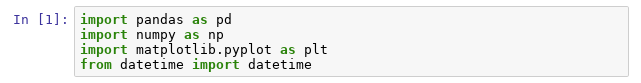
\includegraphics[width=\linewidth]{carga.png}\\
\end{figure}
%%%%%%%%%%%%%%%%%%%%%%%%%%
Después leí cada archivo csv por separado.\\
\begin{figure}[H]
	\centering
    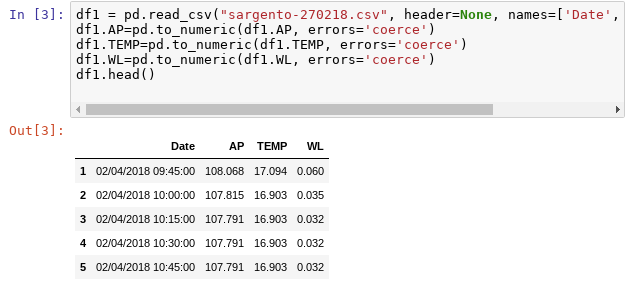
\includegraphics[width=\linewidth]{leer1.png}\\
\end{figure}
\begin{figure}[H]
	\centering
    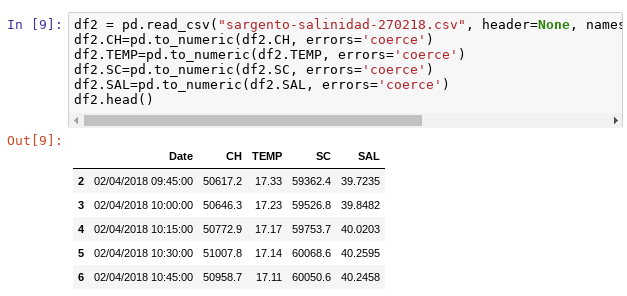
\includegraphics[width=\linewidth]{leer2.png}\\
\end{figure}
%%%%%%%%%%%%%%%%%%%%%
Después numeré el mes de cada archivo.\\
\begin{figure}[H]
	\centering
    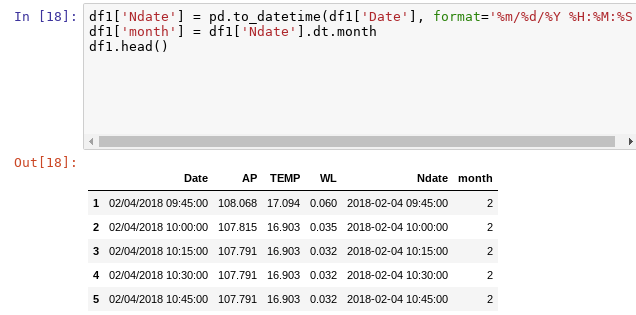
\includegraphics[width=\linewidth]{mes1.png}\\
\end{figure}
\begin{figure}[H]
	\centering
    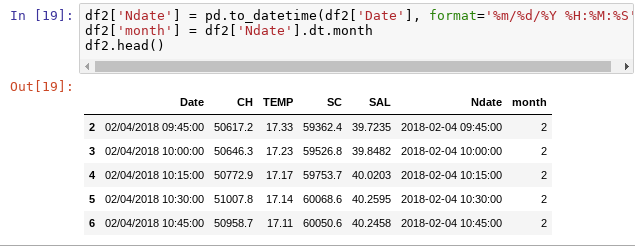
\includegraphics[width=\linewidth]{mes2.png}\\
\end{figure}
%%%%%%%%%%%%%%%%%%%%%%%%%%%%%%%%
Siguió hacer tres gráficas de caja; mes contra nivel del mar, mes contra salinidad y mes contra temperatura.\\
\begin{figure}[H]
	\centering
    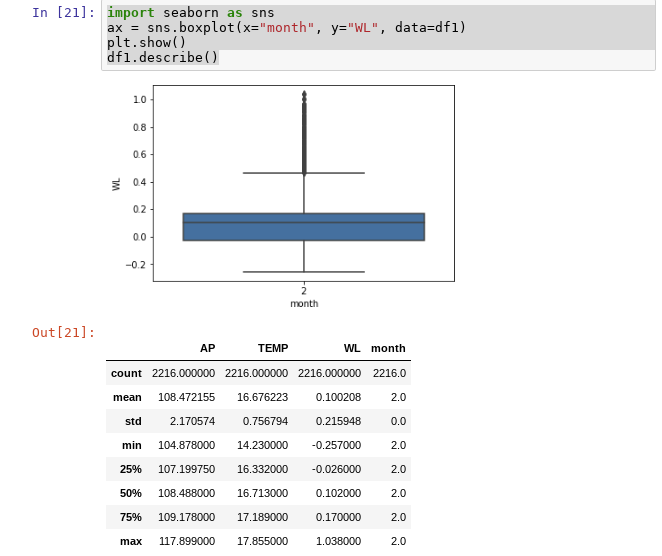
\includegraphics[width=\linewidth]{caja1.png}\\
\end{figure}
\begin{figure}[H]
	\centering
    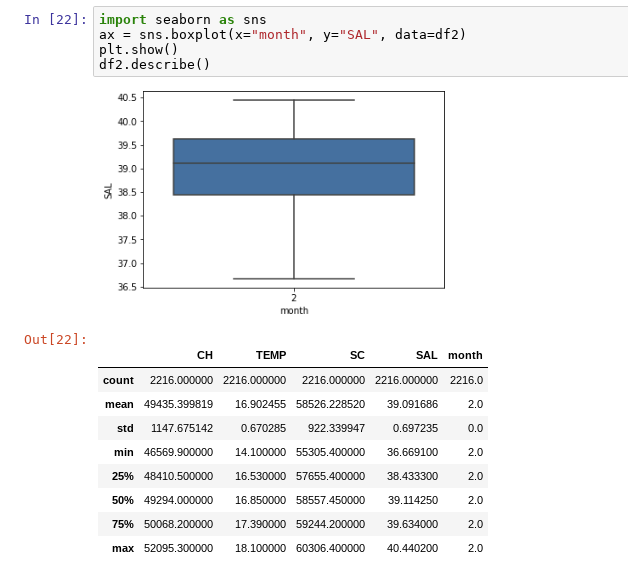
\includegraphics[width=\linewidth]{caja2.png}\\
\end{figure}
\begin{figure}[H]
	\centering
    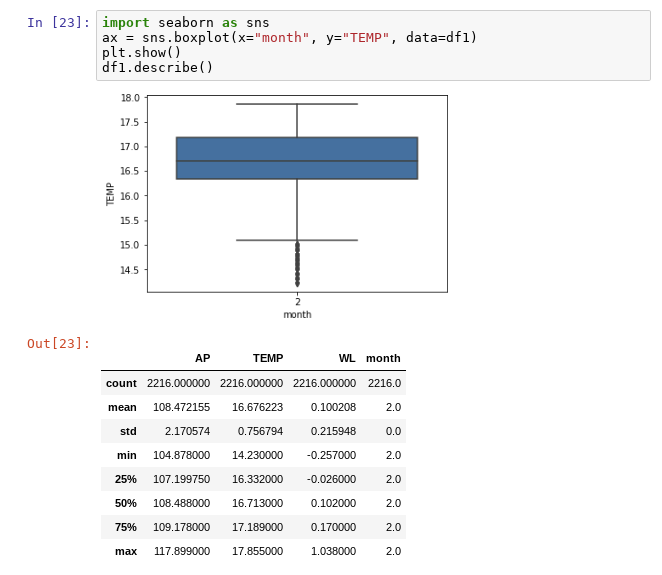
\includegraphics[width=\linewidth]{caja3.png}\\
\end{figure}
%%%%%%%%%%%%%%%
Ahora se pide una gráfica de regresión lineal que relaciones la salinidad con el nivel del mar. Por ésto mismo es necesario crear un nuevo data frame que relacione ambas variables.\\
\begin{figure}[H]
	\centering
    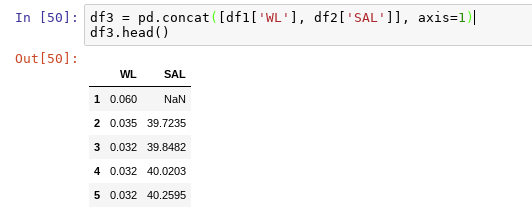
\includegraphics[width=\linewidth]{df3.png}\\
\end{figure}
%%%%%%%%%%%%%%%%%%%
Después realizamos la grafica.\\
\begin{figure}[H]
	\centering
    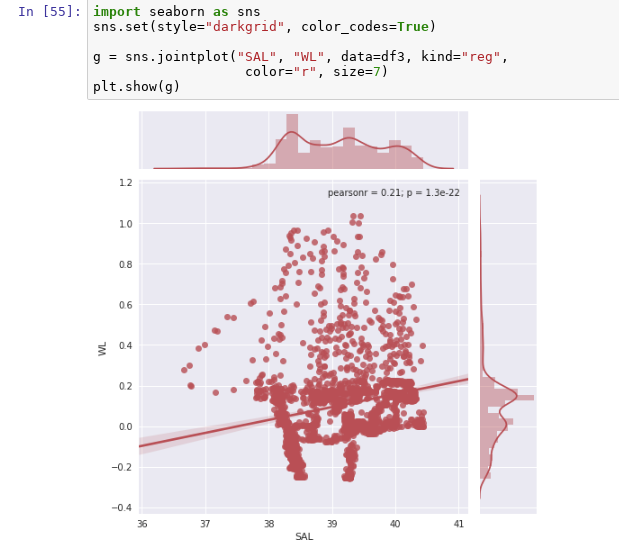
\includegraphics[width=\linewidth]{reg1.png}\\
\end{figure}
Ahora la segunda que relaciona nivel del mar y temperatura.\\
\begin{figure}[H]
	\centering
    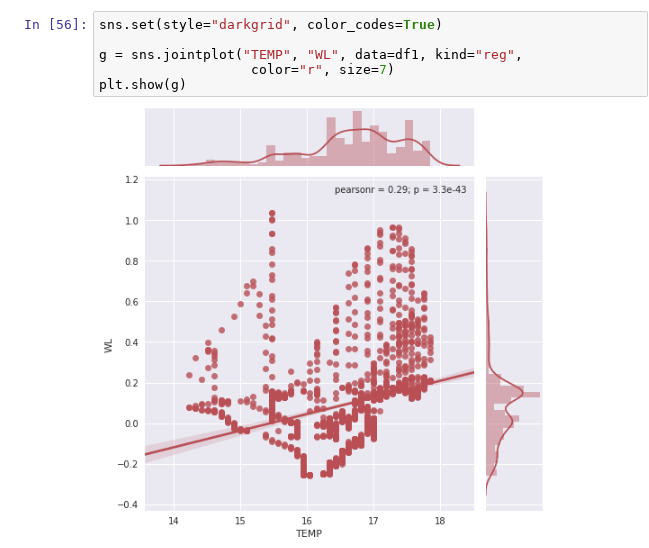
\includegraphics[width=\linewidth]{reg2.png}\\
\end{figure}
Y la que relaciona salinidad y temperatura del agua.
\begin{figure}[H]
	\centering
    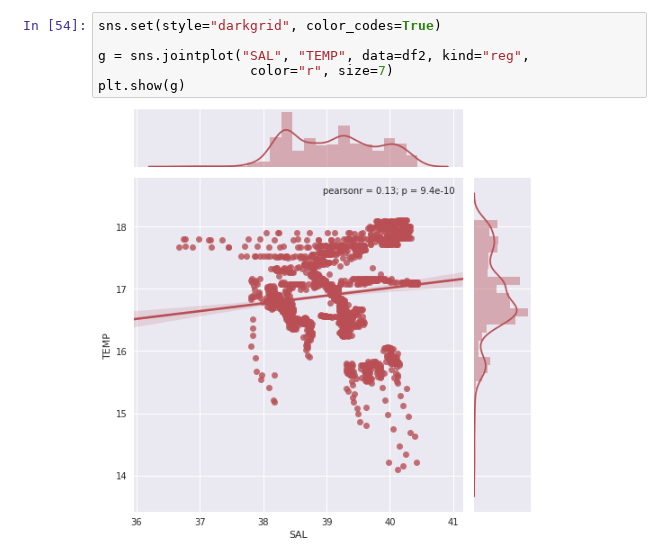
\includegraphics[width=\linewidth]{reg3.png}\\
\end{figure}
Ahora se piden tres graficas con respecto al tiempo: nivel del mar, salinidad y temperatura.\\
\begin{figure}[H]
	\centering
    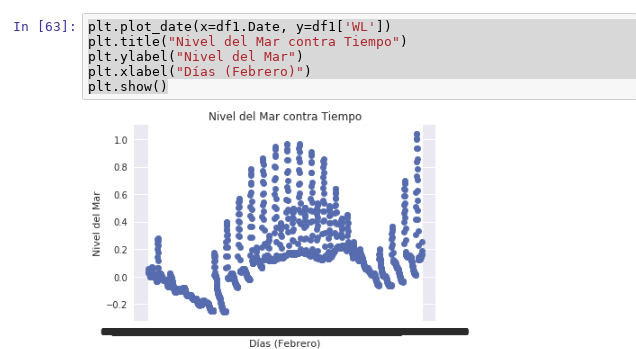
\includegraphics[width=\linewidth]{t1.png}\\
\end{figure}
\begin{figure}[H]
	\centering
    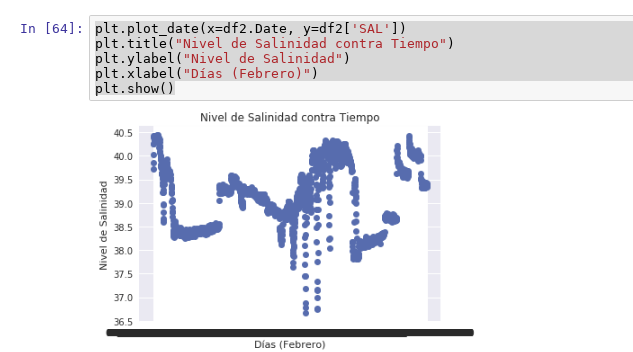
\includegraphics[width=\linewidth]{t2.png}\\
\end{figure}
\begin{figure}[H]
	\centering
    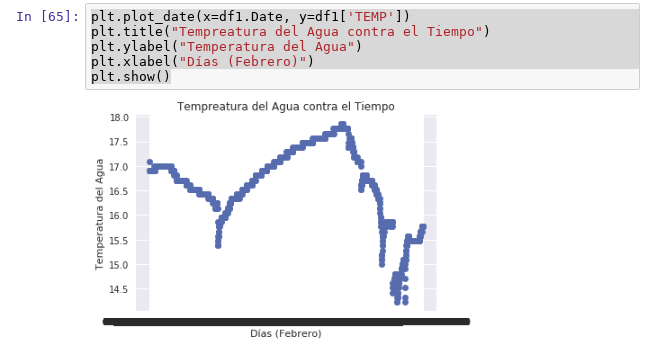
\includegraphics[width=\linewidth]{t3.png}\\
\end{figure}
Después debemos hacer dos graficas de superposición en el eje y. La primera de nivel del mar y salinidad, mientras que la segunda de nivel del mar y temperatura del agua.\\
\begin{figure}[H]
	\centering
    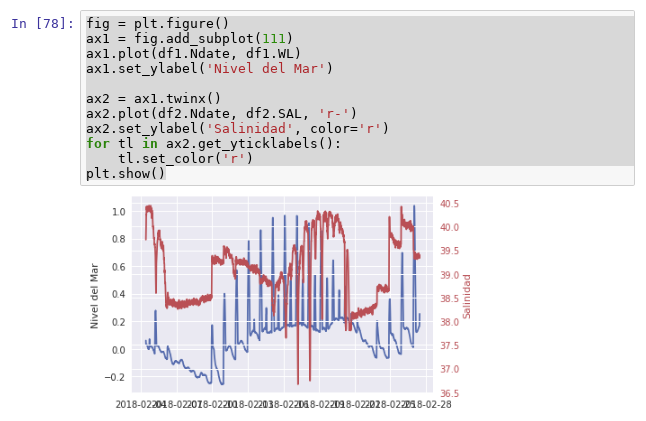
\includegraphics[width=\linewidth]{tw1.png}\\
\end{figure}
\begin{figure}[H]
	\centering
    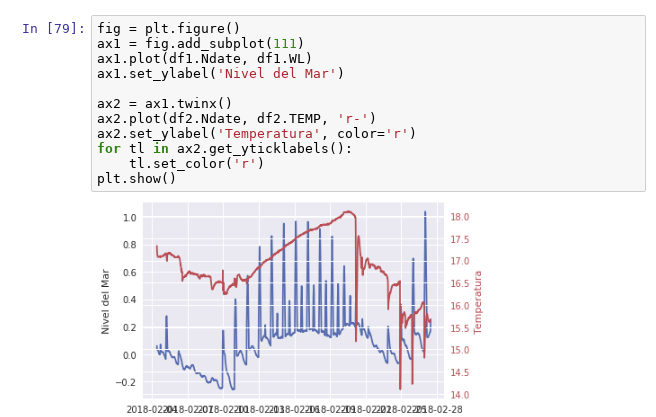
\includegraphics[width=\linewidth]{tw2.png}\\
\end{figure}
Finalmente, debemos hacer utilizar la función xlim de matplotlib para checar si se relacionan el nivel del mar con la salinidad y/o temperatura del agua.\\
\begin{figure}[H]
	\centering
    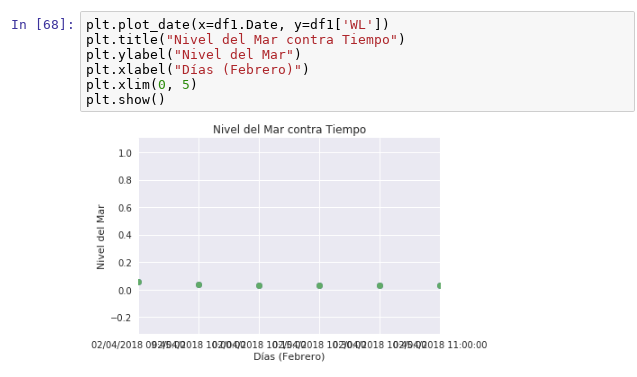
\includegraphics[width=\linewidth]{x1.png}\\
\end{figure}
\begin{figure}[H]
	\centering
    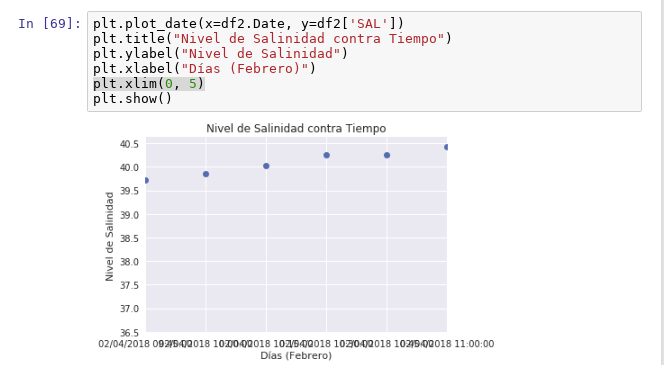
\includegraphics[width=\linewidth]{x2.png}\\
\end{figure}
\begin{figure}[H]
	\centering
    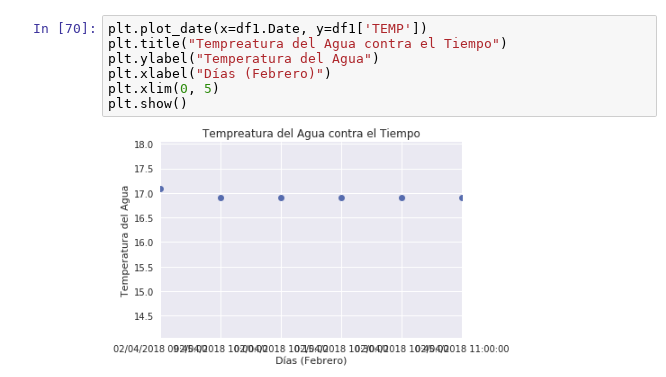
\includegraphics[width=\linewidth]{x3.png}\\
\end{figure}
Tras ésto podemos notar que la salinidad y la temperatura del agua cambian cuando una de éstas variables lo hace. En cuanto a la variable nivel del mar, no pude notar relación alguna.
\end{document}
